\chapter{Conceptualisation and Modelling}
\label{chp2:concept_model}
[provide an overview]

\section{System Concepts}
%WHAT you are going to present in this chapter/section
%WHY you are presenting it, and
%HOW you are going to present it
The report contains many variable names and use of terminology for concepts that is used throughout the report. These variables and terminologies are defined here.\\

The double pendulum is a underactuated system which is defined as a system where the input to the system cannot command all of the state variables an instantaneous acceleration \citeauthor{tedrake}. This is due to the control input only actuating the lower pendulum and the energy in the lower pendulum must be transferred to the upper pendulum to initiate an acceleration. \\

The robotic gymnast is described as a double pendulum consisting out of an actuated- and unactuated pendulum as seen in Figure \ref{fig:doublePen}. The position of the unactuated pendulum is described by the angle $\theta$ whereas the actuated pendulum is described by $\phi$ relative to $\theta$. The angle's $\theta$ and $\phi$ are the independent parameters that describe the entire system.\\

There are two position of interest where the system contain special characteristics. These 2 positions are the stable- and unstable equilibrium positions. In the stable position the system is at rest hanging downwards where both $\theta$ and $\phi = \SI{0}{\radian}$. It is stable due to the system containing negative real poles resulting in the system returning to this position when disturbed. The unstable equilibrium position is where $\theta=\SI{2\pi}{\radian}$ and $\phi = \SI{0}{rad}$ resulting in the robotic gymnast balancing in the inverted position. In this position the system contains positive real poles and any disturbance will cause the system to grow away from this position.\\


\begin{comment}
region of controllability:he null controllability region is the set of states that can be steered to inverted unstable equilibrium position in a fixed time with a constrained control input \cite{null_controllability}.
LTI system
\end{comment}



\section{Mathematical Model}
\label{sec:mathematical_model}
%WHAT you are going to present in this chapter/section
%WHY you are presenting it, and
%HOW you are going to present it
\begin{figure}[h]
	\centering
	
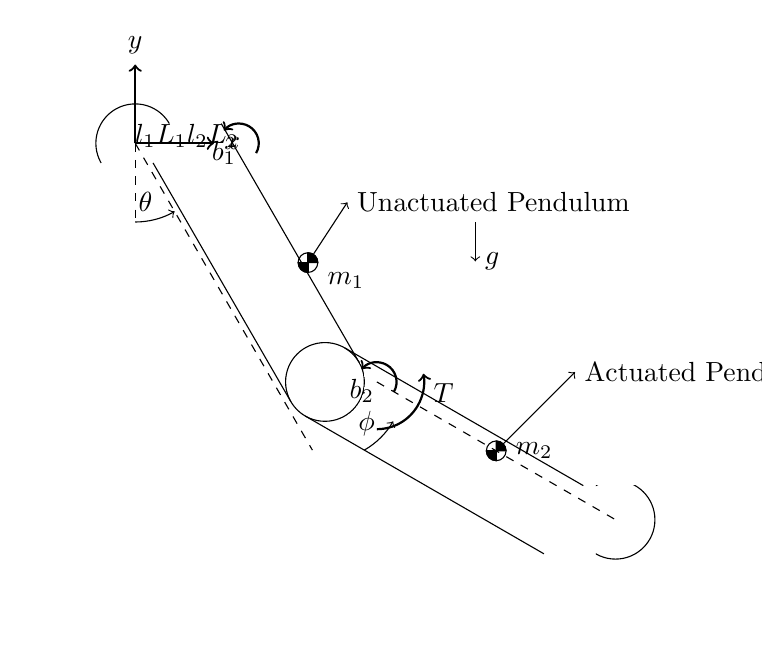
\begin{tikzpicture}[scale=0.5]

\begin{scope}
\clip [rotate=30] (-2,0) rectangle (2,2);
\draw (0,0) circle [radius=1cm];
\end{scope}

\coordinate (O) at (0,0) ;
% Second cirle middle point
\coordinate (A) at (3.5,-6.06217); 
\coordinate (B) at (3.5+6.06217,-6.06217-3.5); 
	% Lenght of pendulums are 7cm

	% Axis for underactuated Pendulum
	\draw[->,thick] (0,0) -- (2,0) node[anchor=west] {$x$};
	\draw[->,thick] (0,0) -- (0,2) node[anchor=south] {$y$};
	\draw[dashed] (0,0) -- (0,-2);
	
	%%%%%%%%%%%%%%%%%%%%%%%%%%%%%%%%%%%%%%%%%%%%%%%%%%%%%%%%%%%%%%%%%%%%%%%%%%%%%%
							%% Theta %%
	\begin{scope}
		\draw[->] (0,-2) arc (270:300:2);
		\draw (280:1.5) node {$\theta$};
	\end{scope}
	%%%%%%%%%%%%%%%%%%%%%%%%%%%%%%%%%%%%%%%%%%%%%%%%%%%%%%%%%%%%%%%%%%%%%%%%%%%%%%
	
	%%%%%%%%%%%%%%%%%%%%%%%%%%%%%%%%%%%%%%%%%%%%%%%%%%%%%%%%%%%%%%%%%%%%%%%%%%%%%%
				%% Middle line for underactuated pendulum %%
	\draw[dashed] (0,0) -- (4.5,-7.79422);
	%%%%%%%%%%%%%%%%%%%%%%%%%%%%%%%%%%%%%%%%%%%%%%%%%%%%%%%%%%%%%%%%%%%%%%%%%%%%%%
	
		
	%%%%%%%%%%%%%%%%%%%%%%%%%%%%%%%%%%%%%%%%%%%%%%%%%%%%%%%%%%%%%%%%%%%%%%%%%%%%%%
					%% Dimensions of underactuated Pendulum %%
	\dimline[line style = {line width=0.7},extension start length=-0.25, extension end length=-0.4]{(-1.732,-1)}{(-1.732+1.75,-1-3.031)}{$l_{1}$}
	
	\dimline[line style = {line width=0.7},extension start length=-0.25, extension end length=-0.25]{(-2.598,-1.5)}{(-2.598+3.5,-1.5-6.06217)}{$L_{1}$}
	
	%%%%%%%%%%%%%%%%%%%%%%%%%%%%%%%%%%%%%%%%%%%%%%%%%%%%%%%%%%%%%%%%%%%%%%%%%%%%%%

	%Long lines for underactuated pendulum
	\draw (0.8660,0.5) -- (0.866+3.5,0.5-6.06217);
	\draw (-0.8660,-0.5) -- (-0.866+3.5,-0.5-6.06217);	
	
	
	
	%%%%%%%%%%%%%%%%%%%%%%%%%%%%%%%%%%%%%%%%%%%%%%%%%%%%%%%%%%%%%%%%%%%%%%%%%%%%%%
					%% Middle circle for both pendulums %%
	\begin{scope}
		%\clip [rotate=00] (0.866+3.5,0.5-6.06217+2) rectangle (-0.866+3.5-2,-0.5-6.06217);
	\clip (A) circle [radius=1.02];
	\draw (A) circle [radius=1cm];
	\end{scope}
	
	%\draw [rotate=00] (0.866+3.5,0.5-6.06217+2) rectangle (-0.866+3.5-2,-0.5-6.06217);
	
	%%%%%%%%%%%%%%%%%%%%%%%%%%%%%%%%%%%%%%%%%%%%%%%%%%%%%%%%%%%%%%%%%%%%%%%%%%%%%%
	% Axis for lower Pendulum
	%\draw[->,thick] (3.5,-6.06217) -- (6.5,-6.06217) node[anchor=west] {$x_{2}$};
	%\draw[->,thick] (3.5,-6.06217) -- (3.5,-3.06217) node[anchor=south] {$y_{2}$};
	%\draw[dashed] (3.5,-6.06217) -- (3.5,-8.56217);
	
	% Long lines for actuated pendulum
	\draw (3.5+0.5,-6.06217+0.86602) -- (3.5+0.5+6.06217,-6.06217+0.86602-3.5);
	\draw (3.5-0.5,-6.06217-0.86602) -- (3.5-0.5+6.06217,-6.06217-0.86602-3.5);
	
	%%%%%%%%%%%%%%%%%%%%%%%%%%%%%%%%%%%%%%%%%%%%%%%%%%%%%%%%%%%%%%%%%%%%%%%%%%%%%%
							%%  Phi %%
	\begin{scope}
	\draw[->] (4.5,-7.79422) arc (300:330:2);
	
	
	\draw (3.5,-6.06217)+ (315:1.5) node {$\phi$};
	\end{scope}
	%%%%%%%%%%%%%%%%%%%%%%%%%%%%%%%%%%%%%%%%%%%%%%%%%%%%%%%%%%%%%%%%%%%%%%%%%%%%%%
	
	%%%%%%%%%%%%%%%%%%%%%%%%%%%%%%%%%%%%%%%%%%%%%%%%%%%%%%%%%%%%%%%%%%%%%%%%%%%%%%
						%% Dimensions of actuated Pendulum %%
	\dimline[line style = {line width=0.7},extension start length=-0.25, extension end length=-0.4]{(2.5,-7.79421)}{(5.53108,-9.54422)}{$l_{2}$}
	
	\dimline[line style = {line width=0.7},extension start length=-0.25, extension end length=-0.25]{(2,-8.66028)}{(8.06217,-12.1602)}{$L_{2}$}
	
	%%%%%%%%%%%%%%%%%%%%%%%%%%%%%%%%%%%%%%%%%%%%%%%%%%%%%%%%%%%%%%%%%%%%%%%%%%%%%%

	
	%%%%%%%%%%%%%%%%%%%%%%%%%%%%%%%%%%%%%%%%%%%%%%%%%%%%%%%%%%%%%%%%%%%%%%%%%%%%%%
							%% Circle at the bottom %%
	\begin{scope}
	\clip [rotate=00] (3.5+0.5+6.06217+2,-6.06217+0.86602-3.5) rectangle ((3.5-0.5+6.06217,-6.06217-0.86602-3.5-2);
	\draw (B) circle [radius=1cm];
	\end{scope}
	%%%%%%%%%%%%%%%%%%%%%%%%%%%%%%%%%%%%%%%%%%%%%%%%%%%%%%%%%%%%%%%%%%%%%%%%%%%%%%

	
	%%%%%%%%%%%%%%%%%%%%%%%%%%%%%%%%%%%%%%%%%%%%%%%%%%%%%%%%%%%%%%%%%%%%%%%%%%%%%%
					%% Middle line for actuated pendulum %%
	\draw[dashed] (3.5,-6.06217)--(3.5+6.06217,-6.06217-3.5);
	%%%%%%%%%%%%%%%%%%%%%%%%%%%%%%%%%%%%%%%%%%%%%%%%%%%%%%%%%%%%%%%%%%%%%%%%%%%%%%
		
	%%%%%%%%%%%%%%%%%%%%%%%%%%%%%%%%%%%%%%%%%%%%%%%%%%%%%%%%%%%%%%%%%%%%%%%%%%%%%%
				%% Centroid symbol for underactuade pendulum %%
	\draw (1.75,-3.0310) circle [radius=0.25cm];
	\draw (1.75-0.25,-3.0310) -- (1.75+0.25,-3.0310)  node[below right]{$m_{1}$};`
	\draw (1.75,-3.0310+0.25) -- (1.75,-3.0310-0.25);
	\filldraw[fill=black,draw=black] (1.75,-3.0310) -- (1.75+0.25,-3.0310)
		arc[start angle = 0, end angle = 90, radius = 0.25] -- cycle;
		
	\filldraw[fill=black,draw=black] (1.75,-3.0310) -- (1.75-0.25,-3.0310)
	arc[start angle = 180, end angle = 270, radius = 0.25] -- cycle ;
	%%%%%%%%%%%%%%%%%%%%%%%%%%%%%%%%%%%%%%%%%%%%%%%%%%%%%%%%%%%%%%%%%%%%%%%%%%%%%%
	
	%%%%%%%%%%%%%%%%%%%%%%%%%%%%%%%%%%%%%%%%%%%%%%%%%%%%%%%%%%%%%%%%%%%%%%%%%%%%%%
				%% Centroid symbol for actuaded pendulum %%
	\draw (6.53108,-7.81217) circle [radius=0.25cm];
	\draw (6.53108-0.25,-7.81217) -- (6.53108+0.25,-7.81217)  node[right]{$m_{2}$};
	\draw (6.53108,-7.81217+0.25) -- (6.53108,-7.81217-0.25);
	\filldraw[fill=black,draw=black] (6.53108,-7.81217) -- (6.53108+0.25,-7.81217)
	arc[start angle = 0, end angle = 90, radius = 0.25] -- cycle;
	
	\filldraw[fill=black,draw=black] (6.53108,-7.81217) -- (6.53108-0.25,-7.81217)
	arc[start angle = 180, end angle = 270, radius = 0.25] -- cycle ;
	%%%%%%%%%%%%%%%%%%%%%%%%%%%%%%%%%%%%%%%%%%%%%%%%%%%%%%%%%%%%%%%%%%%%%%%%%%%%%%
	
	% Torque Input
	%\draw[->,thick] (3.5,-7.5) to [bend right] (5.25,-4.76314) node[right]{$T$}; 
	\draw[->,thick] (A) +(0,-1.2) arc (270:370:1.2) node[below right] {$T$};
	
	
	% Damping in bearings
	\draw[->,thick] (0.433,-0.25) arc (330:500:0.5) node[below] {$b_{1}$};
	
	% Damping between motor rotor and stator 
	\draw[->,thick] (A)+(0.433,-0.25) arc (330:500:0.5) node[below] {$b_{2}$};
	
	% Direction of gravity
	\draw[->] (6,-2)--(6,-3) node[right]{$g$};
	
	% Labels for pendulums
	\draw[->] (1.75,-3.0310)--(2.75,-1.5) node[right]{Unactuated Pendulum};
	\draw[->] (6.53108,-7.81217)--(8.53108,-5.81217) node[right]{Actuated Pendulum};
	
	
\end{tikzpicture}
	\caption{Free Body Diagram of the Double Pendulum}
	\label{fig:doublePen}
\end{figure}

The approach taken to derive the mathematical model of the robotic gymnast is presented in this section. It is presented to allow the reader to understand parameters used throughout the report and critical to the implementation of the swing-up controller. The swinging of the robotic gymnast consists of non-linear behaviour and is required to fully derive the dynamics of the system. The detailed mathematical derivations are available in Appendix \ref{sec:math_model}. A summary of the motivation and paradigm approach to the derivation is provided here.\\

 Figure \ref{fig:doublePen} shows the free body diagram of the robotic gymnast which was modelled as two pendulums connected together with a hinge. Each pendulum was modelled as having their mass distributed arbitrary along their axis. A torque is actuating the lower pendulum and friction was modelled as a function of the angular velocity.\\

The Euler-Lagrange equation shown in (\ref{eq:euler_lagrange_expanded}) was used to derive the dynamics of the system by analysing the energy of the system which is easily defined as the potential energy $T$ and the kinetic energy $V$ of the 2 pendulums.
 
\begin{equation} \label{eq:euler_lagrange_expanded}
\frac{d}{dt}\frac{\partial\mathcal{L}}{\partial\vec{\dot{q}}}-\frac{\partial\mathcal{L}}{ \vec{\partial q}} = 0
\end{equation}

\begin{equation} \label{eq:euler_lagrane}
\mathcal{L}=T-V
\end{equation}

Using the Euler-Lagrange equation leads to the condense equations shown in (\ref{eq:condense1}) and (\ref{eq:condense2}),
\begin{equation} \label{eq:condense1}
d_{11}\ddot{\theta}+d_{12}\ddot{\phi} + h_{1} + \psi_{1} = 0
\end{equation}
\begin{equation} \label{eq:condense2}
d_{21}\ddot{\theta} + d_{22}\ddot{\phi} + h_{2} + \psi_{2} = \tau
\end{equation}
where the coefficients are defined as
\begin{equation} \label{eq:d11}
d_{11} = I_{a} + I_{b} + m_{2}(L_{1}^2 + l_{2}^2+2L_{1}l_{2}\cos(\phi))
\end{equation}
\begin{equation} \label{eq:d12}
d_{12} = I_{b} +m_{2}(l_{2}^2 L_{1}l_{2}\cos(\phi))
\end{equation}
\begin{equation} \label{eq:h1}
h_{1} = -m_{2}L_{1}l_{2}\sin(\phi)\dot{\phi^2}-2m_{2}L_{1}l_{2}\sin(\phi)\dot{\phi}\dot{\theta}
\end{equation}
\begin{equation} \label{eq:psi1}
\psi_{1} = (m_{2}l_{1}+m_{2}L_{1})g\cos(\theta) + m_{2}l_{2}g\cos(\theta+\phi) + f_{c_{1}}
\end{equation}
\begin{equation} \label{eq:d21}
d_{21}= I_{b}+m_{2}(l_{2}^2+L_{1}l_{2}\cos(\phi))
\end{equation}
\begin{equation} \label{eq:d22}
d_{22}= I_{b}+ m_{2}l_{2}^2
\end{equation}
\begin{equation} \label{eq:h2}
h_{2}= m_{2}L_{1}l_{2}\sin(\phi)\dot{\theta^2}
\end{equation}
\begin{equation} \label{eq:psi2}
\psi_{2}= m_{2}l_{2}g\cos(\theta+\phi) + f_{c_{2}}
\end{equation}

The friction that develops in the pendulums are for now represented by the $f_{c_{1}}$ and $f_{c_{2}}$ terms and will be expanded in the system identification section.

\section{Simulation Model}
\label{sec:simulation_model}
	%WHAT you are going to present in this chapter/section
%WHY you are presenting it, and
%HOW you are going to present it

The mathematical model derived in the previous section was implemented in a simulation program so that the controllers can be tested in simulation. Simulating the model allows the designer to understand how system parameters influence the dynamics of the system and the verification of controllers implemented. It will be presented by discussing the non-linearities added to represent the physical model better.\\

Simulation of the robotic gymnast was done using \textit{MATLAB Simulink}. The differential equations shown in equation (\ref{eq:condense1}) and (\ref{eq:condense2}) were implemented using the \textit{MATLAB Function} box. It was required to write $\ddot{\phi}$ and $\ddot{\theta}$ as the subject in each of the \textit{MATLAB Function} box to allow MATLAB to simulate the model.\\

Non-linear behaviour introduced by sensors and components were added such as saturation of the motor torque, gearbox backlash and quantisation of sensory data. These non-linearities were implemented to allow the simulation to be an acceptable representation of the physical system. The Simulink Model used for simulation is shown in Figure \ref{fig:sim_nonlinearfeedback}.

\begin{figure}[h]
	\centering
	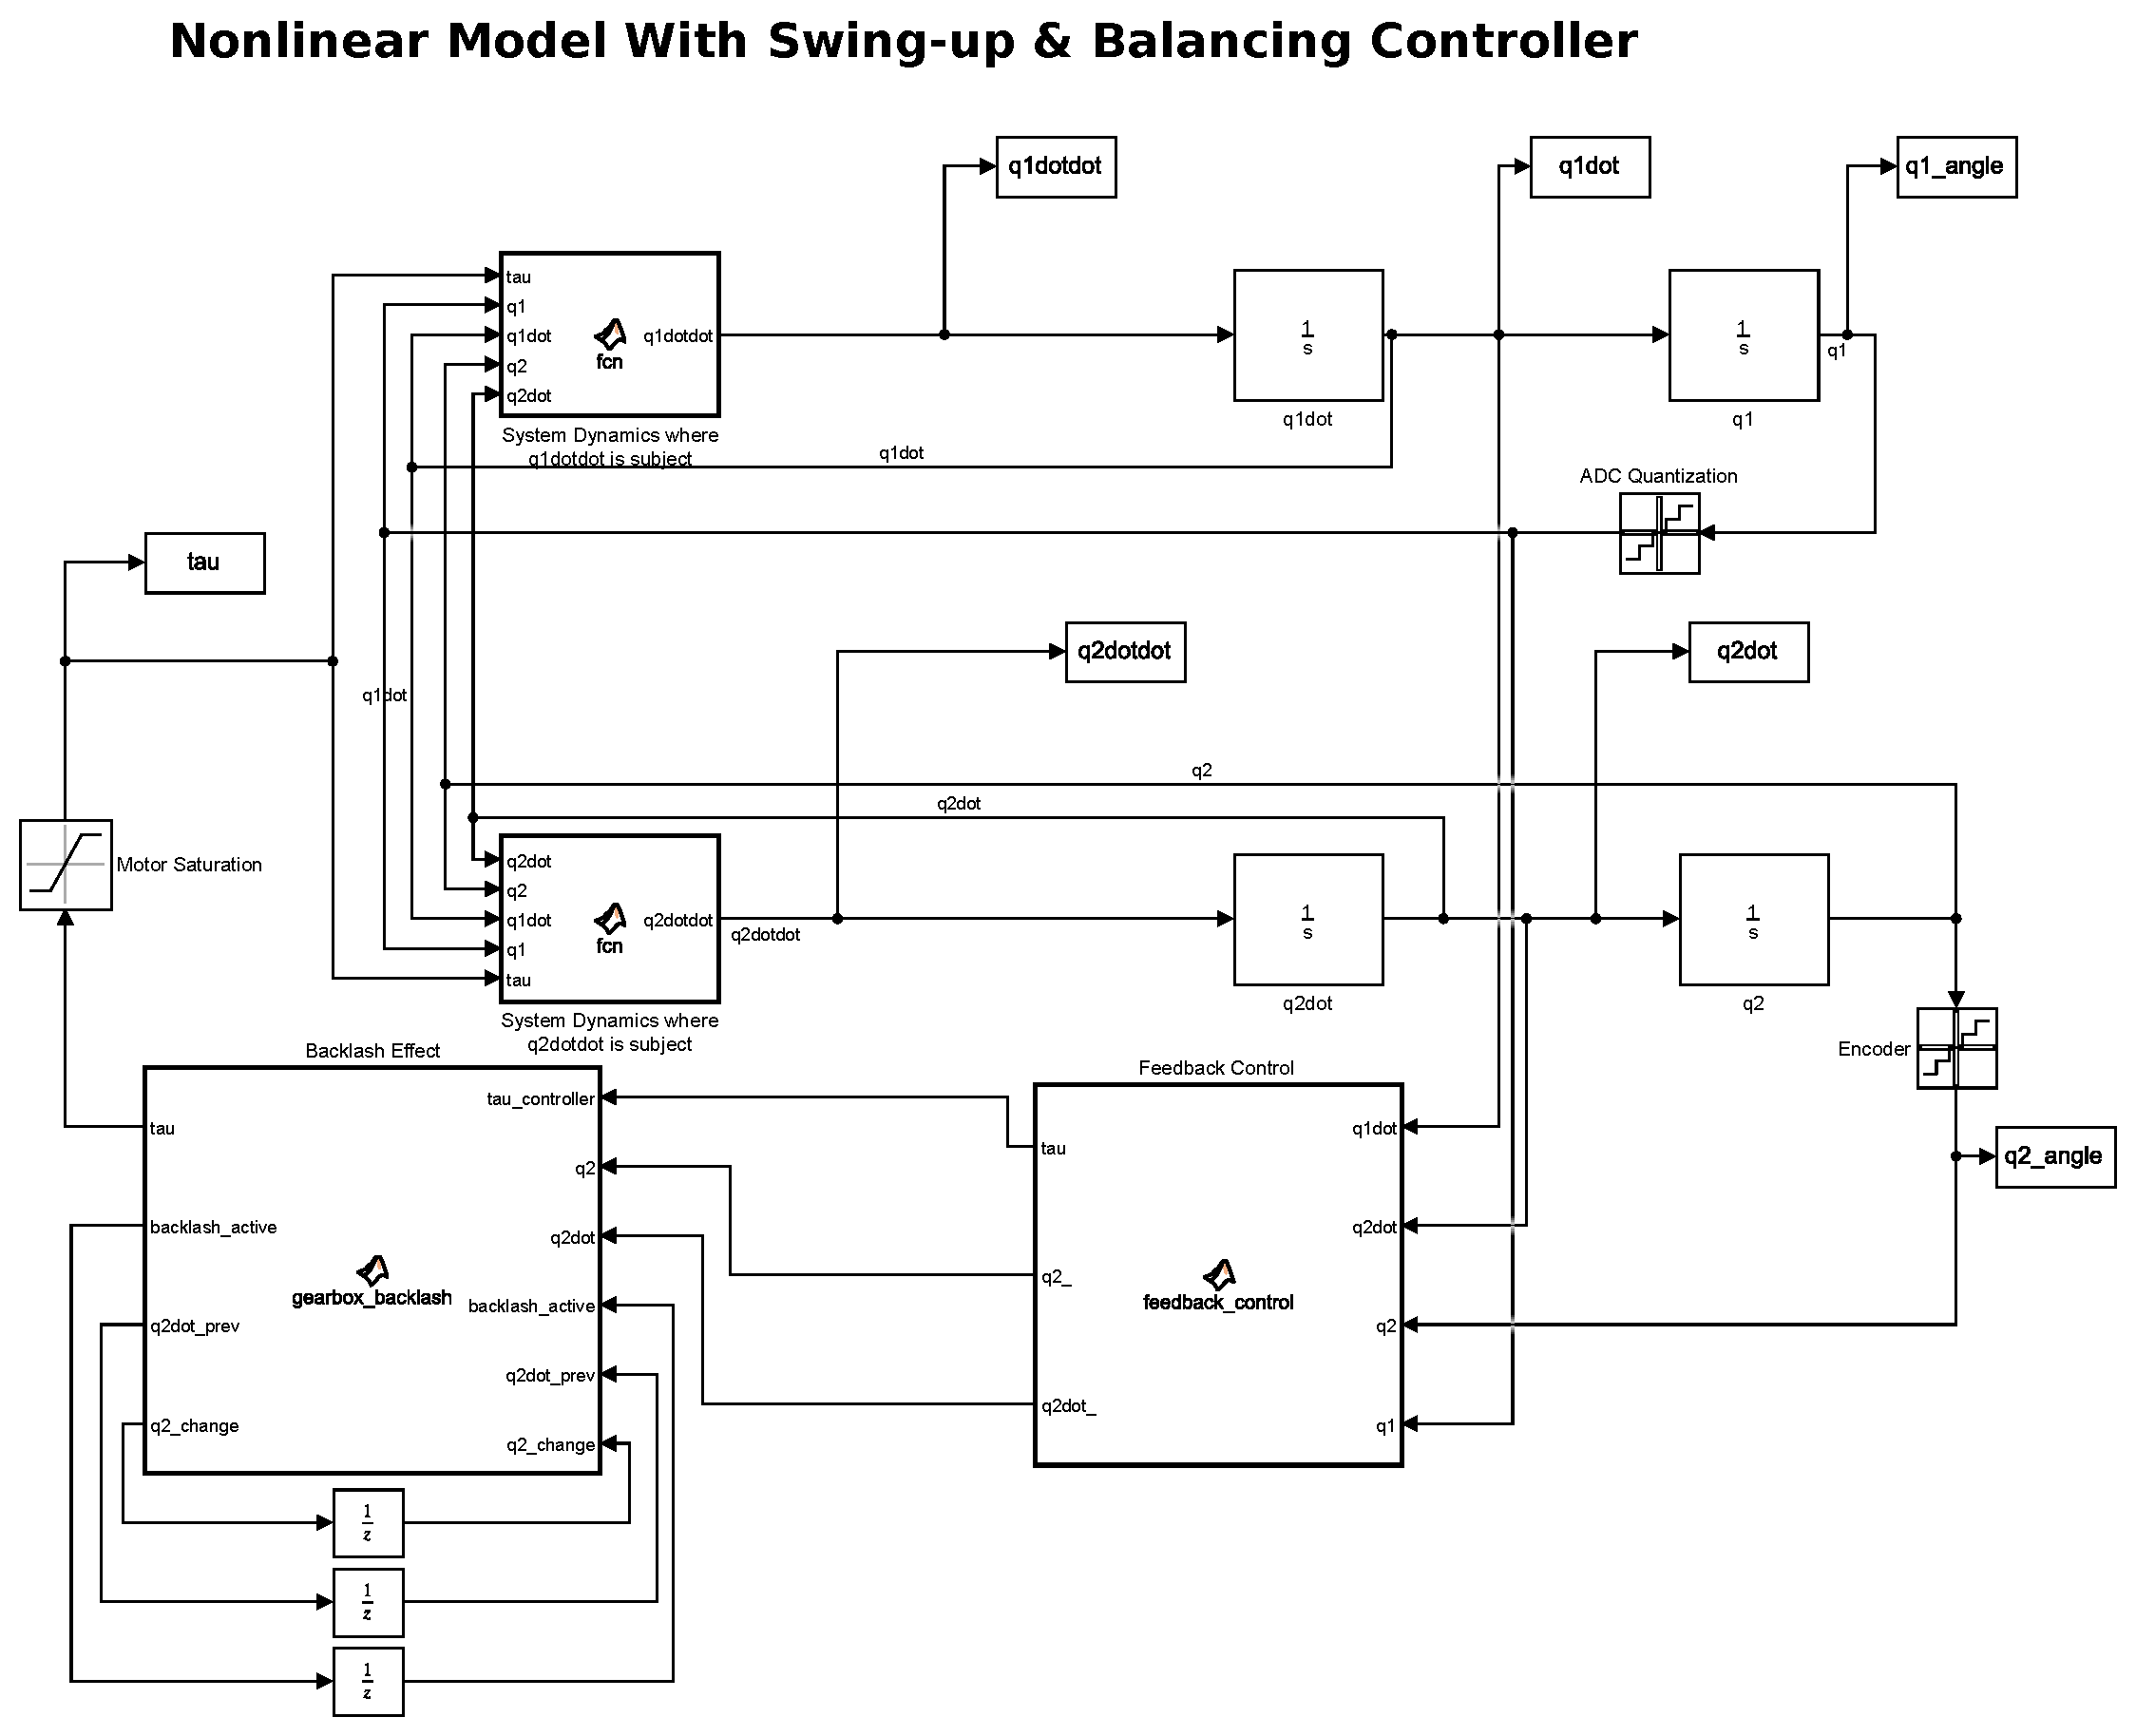
\includegraphics[scale=0.3]{./figs/simulink/latex_simulink.eps}
	\caption{MATLAB Simulink Model}
	\label{fig:sim_nonlinearfeedback}
\end{figure}

\section{System Identification}
\label{sec:system_identification}
%WHAT you are going to present in this chapter/section
%WHY you are presenting it, and
%HOW you are going to present it?

The system identification tests are done to determine the characteristics that describe the behaviour of the system. These characteristics include the damping ratio's and natural frequencies of the system. These characteristics will be presented by showing measured responses and how these responses can be modelled. \\

The project started off with a previous physical model which provided realistic system parameters to allow the simulation to be an acceptable representation of a physical model. From using these previous system parameters the simulation provided a set of specifications for the new mechanical design. All responses shown and values calculated are based on the new mechanical design parameters shown in Table \ref{table:system_param}.\\


		\begin{table}[]
	\centering
	\begin{tabular}{|c|c|}
		\hline
		System Parameter & Value \\
		\hline
		\hline
		$L_{1}$ & \SI{0.235}{m} \\
		\hline
		$L_{2}$ & \SI{0.314}{m} \\ 
		\hline
		$I_{A}$ & \SI{ 0.0022}{kg\cdot m^2}\\
		\hline
		$I_{B}$ & \SI{0.0054}{kg\cdot m^2}\\
		\hline
		$m_{1}$ & \SI{0.576}{kg}\\
		\hline
		$m_{2}$ & \SI{0.492}{kg} \\
		\hline
		$l_{1}$ & \SI{0.205}{m}\\
		\hline
		$l_{2}$ & \SI{0.238}{m}\\
		\hline
	\end{tabular}
	\caption{System Parameters}
	\label{table:system_param}
\end{table}


The system is described by two independent parameters and is expected to contain two natural frequencies each accompanied by a damping coefficient. The first natural frequency of the system was determined by inspecting the response of the system when starting at an initial condition and keeping $\phi = \SI{0}{\radian}$ throughout the response. This was done by using a lightweight PVC pipe that has negligible effect on the weight of the system. The actuated pendulum and unactuated pendulum are constrained to this pipe to ensure the two pendulums stay in-line with each other and thus ensuring $\phi = \SI{0}{\radian}$. The response of the system is shown in Figure \ref{fig:q1_response} starting at an initial condition of roughly $\theta = \frac{\pi}{6}$. The accuracy of the initial conditions is of little importance, but must allow the response to contain a few oscillations to accurately determine the parameter of interest.\\

\begin{figure}[h]
	\centering
	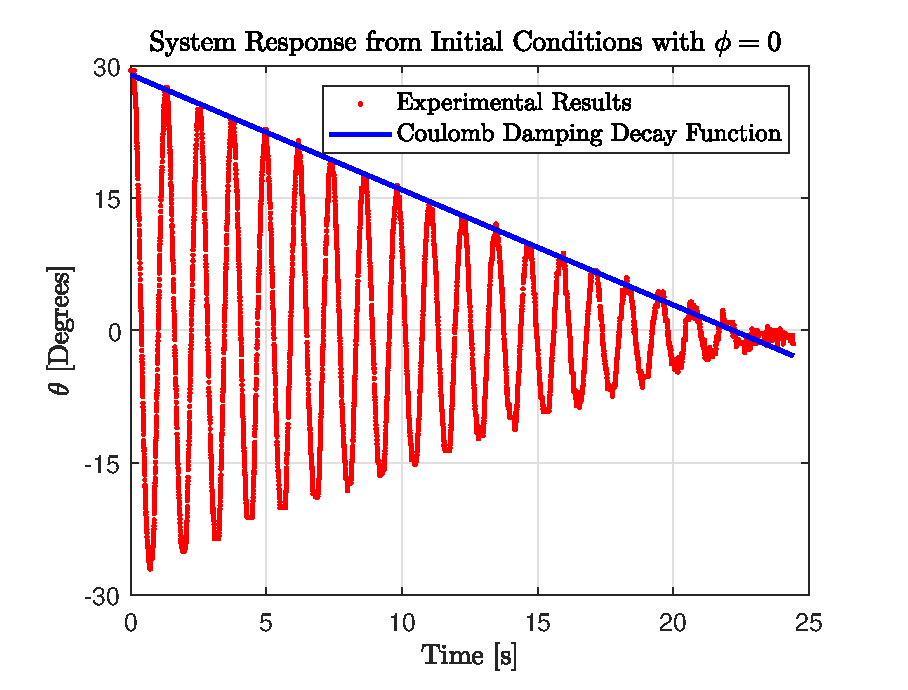
\includegraphics[scale=1]{./figs/q1_initial_response.eps}
	\caption{Initial Condition System Response while $ \phi = \SI{0}{rad} $ }
	\label{fig:q1_response}
\end{figure}


The second natural frequency was determined by analysing the response of the system when $\phi$ starts at an initial condition and keeping $\theta = \SI{0}{\radian}$ throughout the response. This was accomplished by constraining the unactuated pendulum using hard stops. Figure \ref{fig:q2_response} shows the measured response of the system when $\phi$ starts at an initial condition and keeping $\theta = \SI{0}{\radian} $.\\

\begin{figure}[h]
	\centering
	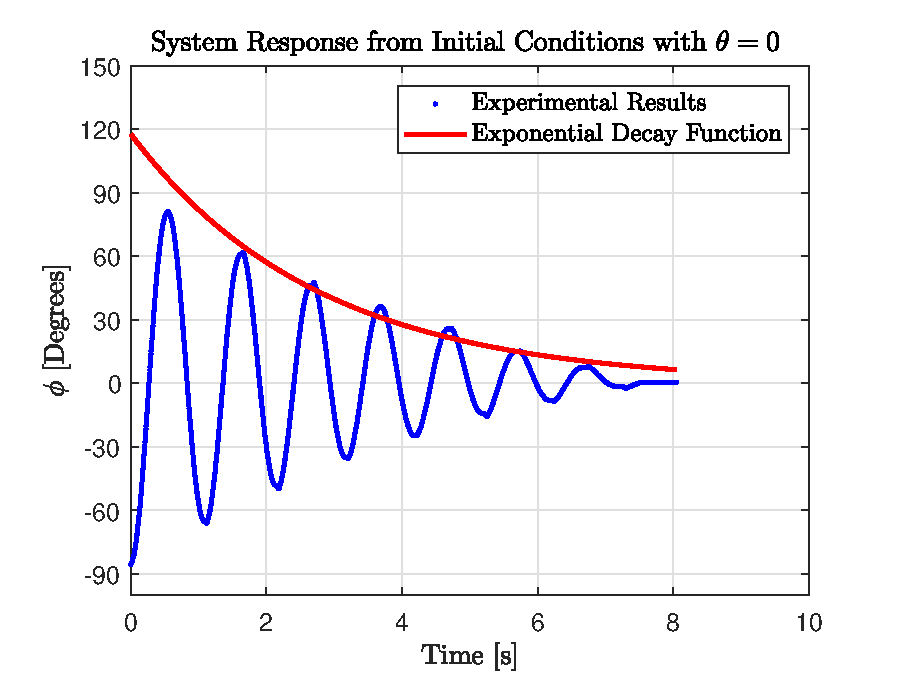
\includegraphics[scale=1]{./figs/q2_initial_response.eps}
	\caption{Initial Condition System Response while $ \theta = \SI{0}{rad} $ }
	\label{fig:q2_response}
\end{figure}

The responses shown in Figure \ref{fig:q1_response} and \ref{fig:q2_response} can be characterised as equation (X) where the frequency of oscillation is caused by the damped natural frequency. This damped natural frequency was determined by measuring the time difference between peaks. The practical results contains a variation on the time difference between peaks and thus the mean of the time differences were calculated and shown in Table \ref{table:system_characteristic}.\\

The friction torques, $f_{c_{1}}$ and $f_{c_{2}}$ that were set as unknowns in the derivation of the robotic gymnast will be expanded on in the following section by analysing how the decaying of the responses can be characterised.\\

The response shown in Figure \ref{fig:q1_response} is under the influence of coulomb damping due to the response being characterised by the amplitude decaying linearly with a constant slope. Coulomb damping is caused by sliding friction and its torque is opposite to the direction of rotation \citep{coulomb_friction}. It is thus characterised as  $$ f_{c_{1}} = 
\left \{
\begin{tabular}{cc}
$ -\mu N $ & $ \dot{\theta}> 0 $\\
$ 0 $ & $ \dot{\theta} = 0$\\
$\mu N$ &   $ \dot{\theta} < 0$ \\
\end{tabular}
\right \}
$$

It is shown in \citet{coulomb_friction} that the slope is defined as 
\begin{equation} \label{eq:coulomb_slope}
-\frac{2\mu N \omega_{n}}{\pi mg}
\end{equation}

where $N$  is the normal force. The slope seen in the decay function in Figure \ref{fig:q1_response} was calculated using linear regression and by knowing the terms in equation (\ref{eq:coulomb_slope}) the combined $\mu N$ term can be calculated as shown in Table \ref{table:system_characteristic}.\\

The response shown in Figure \ref{fig:q2_response} is under the influence of viscous damping due to the amplitude decaying exponentially with time and this behaviour is modelled by the following equation: $$\tau(t) = Ae^{-\zeta \omega_{n}t}$$ where $\omega_{n}$ is the natural frequency, $\zeta$ the damping ratio of the system and $A$ represents the initial amplitude. The damped natural frequencies of the system have already been determined and linear regression was used to determine the best $\zeta$ that will fit the measured data. The decaying function is shown in Figure \ref{fig:q2_response} with the $\zeta$ value shown in Table \ref{table:system_characteristic}. It is visible from the response that the damping ratio fits the data well and only starts to deviate near steady state.\\

The damping moment, $f_{c_{2}}$ that develops between the stator and rotor of the hinge can then be characterised as $2\zeta\omega_{n}(\dot{\phi}-\dot{\theta})$. The subtraction of $\dot{\theta}$ is due to the rotor of the hinge rotating relative to the stator.

\begin{comment}
	\begin{table}{|c|c|c|}
	\centering
	\hline
	System Characteristic & Mean & Standard Deviation\\
	\hline
	\hline
	$ f_{1} $ & \SI{0.906}{Hz} & 0.014 \\
	$ f_{2} $ & \SI{1.081}{Hz} & 0.044 \\ 
	\hline
	$\mu N $ & 3 & 3 \\
	\hline
	$\zeta_{2}$ & 3 & 3 \\
	\hline
	\end{tabular}
	\caption{System Characteristic \& their Statistical Properties from 5 Experiments}
	\label{table:system_characteristic}
	\end{table}
\end{comment}

\section{Model Validation}
%WHAT you are going to present in this chapter/section
%WHY you are presenting it, and
%HOW you are going to present it?
The model implemented in simulation must be able to describe the physical model to an acceptable degree to allow any further developments on the simulated model. The simulated model will be validated by comparing the experimental system characteristic values to those attained in simulation.\\

Table \ref{table:experiment_vs_simulation} shows the experimental values determined in the previous section against the simulation characteristic and indicates the simulation model represents the physical model well.\\

Figure \ref{fig:sim_vs_measured_q1} and \ref{fig:sim_vs_measured_q2} provides a visual verification of which the damping effects are modelled to an acceptable degree. It is visible that the simulated response fits the experimental response well, matching the frequency of oscillation during high velocities and large angles. It is only near steady state where the simulated responses deviates a little. \\\\

Figure \ref{fig:sim_vs_measured_q2} does not describe the damping effect throughout the entire response. This is expected due to the damping force not being constant throughout the response as seen in Figure \ref{fig:q2_response}. The average of the damping coefficients were selected and results in variances.


\begin{table}[]
	\centering
	\begin{tabular}{|c|c|c|c|c|}
		\hline
		System & $\omega_{n_{1}}$  & $\omega_{n_{2}}$  & $\zeta_{1}$ & $\zeta_{2}$ \\
		\hline
		\hline
		Experimental  & 5.692 &  6.793 & & \\
		\hline
		Simulation & 5.654 & 6.704 & & \\ 
		\hline
	\end{tabular}
	\caption{Experimental Characteristics vs Simulation Model Characteristic}
	\label{table:experiment_vs_simulation}
\end{table}

\begin{figure}[h]
	\centering
	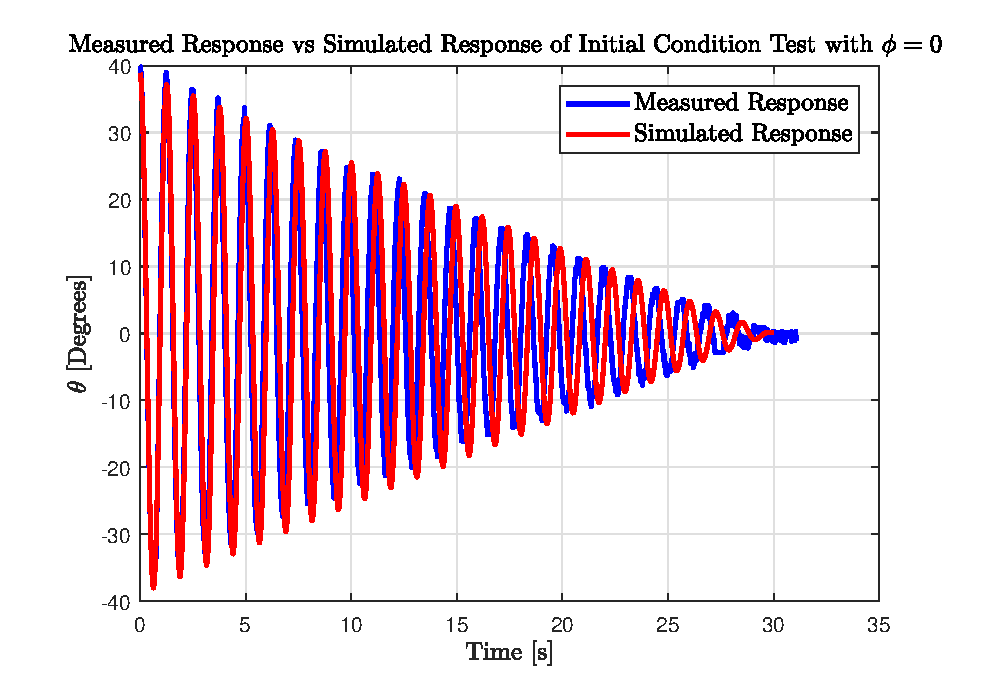
\includegraphics[scale=1]{./figs/sim_vs_measured_q1.eps}
	\caption{Comparison between Simulated and Measured Response with $\phi = \SI{0}{\radian}$ throughout}
	\label{fig:sim_vs_measured_q1}
\end{figure}

\begin{figure}[h]
	\centering
	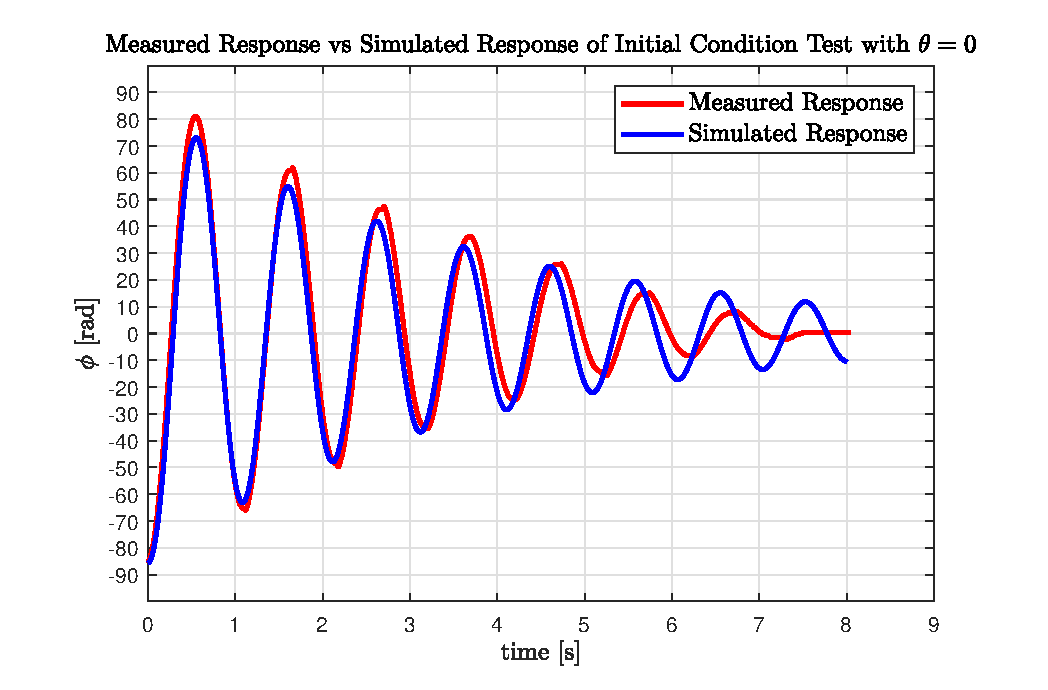
\includegraphics[scale=1]{./figs/sim_vs_measured_q2.eps}
	\caption{Comparison between Simulated and Measured Response with $\theta = \SI{0}{\radian}$ throughout}
	\label{fig:sim_vs_measured_q2}
\end{figure}


